%%%%%%%%%%%%%%%%%%%%%%%%%%%%%%%%%%%%%%%%%
% The Legrand Orange Book
% LaTeX Template
% Version 2.3 (8/8/17)
%
% This template has been downloaded from:
% http://www.LaTeXTemplates.com
%
% Original author:
% Mathias Legrand (legrand.mathias@gmail.com) with modifications by:
% Vel (vel@latextemplates.com)
%
% License:
% CC BY-NC-SA 3.0 (http://creativecommons.org/licenses/by-nc-sa/3.0/)
%
% Compiling this template:
% This template uses biber for its bibliography and makeindex for its index.
% When you first open the template, compile it from the command line with the 
% commands below to make sure your LaTeX distribution is configured correctly:
%
% 1) pdflatex main
% 2) makeindex main.idx -s StyleInd.ist
% 3) biber main
% 4) pdflatex main x 2
%
% After this, when you wish to update the bibliography/index use the appropriate
% command above and make sure to compile with pdflatex several times 
% afterwards to propagate your changes to the document.
%
% This template also uses a number of packages which may need to be
% updated to the newest versions for the template to compile. It is strongly
% recommended you update your LaTeX distribution if you have any
% compilation errors.
%
% Important note:
% Chapter heading images should have a 2:1 width:height ratio,
% e.g. 920px width and 460px height.
%
%%%%%%%%%%%%%%%%%%%%%%%%%%%%%%%%%%%%%%%%%

%----------------------------------------------------------------------------------------
%	PACKAGES AND OTHER DOCUMENT CONFIGURATIONS
%----------------------------------------------------------------------------------------

\documentclass[11pt,fleqn]{book} % Default font size and left-justified equations
\usepackage{svg}
\usepackage{amsmath}
\usepackage{float}
\setlength{\parindent}{2em}
\setlength{\parskip}{1em}
%----------------------------------------------------------------------------------------

%%%%%%%%%%%%%%%%%%%%%%%%%%%%%%%%%%%%%%%%%
% The Legrand Orange Book
% Structural Definitions File
% Version 2.0 (9/2/15)
%
% Original author:
% Mathias Legrand (legrand.mathias@gmail.com) with modifications by:
% Vel (vel@latextemplates.com)
% 
% This file has been downloaded from:
% http://www.LaTeXTemplates.com
%
% License:
% CC BY-NC-SA 3.0 (http://creativecommons.org/licenses/by-nc-sa/3.0/)
%
%%%%%%%%%%%%%%%%%%%%%%%%%%%%%%%%%%%%%%%%%

%----------------------------------------------------------------------------------------
%	VARIOUS REQUIRED PACKAGES AND CONFIGURATIONS
%----------------------------------------------------------------------------------------

\usepackage[top=3cm,bottom=3cm,left=3cm,right=3cm,headsep=10pt,a4paper]{geometry} % Page margins

\usepackage{graphicx} % Required for including pictures
\graphicspath{{Pictures/}} % Specifies the directory where pictures are stored

\usepackage{lipsum} % Inserts dummy text

\usepackage{tikz} % Required for drawing custom shapes

\usepackage[english]{babel} % English language/hyphenation

\usepackage{enumitem} % Customize lists
\setlist{nolistsep} % Reduce spacing between bullet points and numbered lists

\usepackage{booktabs} % Required for nicer horizontal rules in tables

\usepackage{xcolor} % Required for specifying colors by name
\definecolor{ocre}{RGB}{225,100,225} % Define the orange color used for highlighting throughout the book

%----------------------------------------------------------------------------------------
%	FONTS
%----------------------------------------------------------------------------------------

\usepackage{avant} % Use the Avantgarde font for headings
%\usepackage{times} % Use the Times font for headings
\usepackage{mathptmx} % Use the Adobe Times Roman as the default text font together with math symbols from the Sym­bol, Chancery and Com­puter Modern fonts

\usepackage{microtype} % Slightly tweak font spacing for aesthetics
\usepackage[utf8]{inputenc} % Required for including letters with accents
\usepackage[T1]{fontenc} % Use 8-bit encoding that has 256 glyphs

%----------------------------------------------------------------------------------------
%	BIBLIOGRAPHY AND INDEX
%----------------------------------------------------------------------------------------

\usepackage[style=numeric,citestyle=numeric,sorting=nyt,sortcites=true,autopunct=true,babel=hyphen,hyperref=true,abbreviate=false,backref=true,backend=biber]{biblatex}
\addbibresource{bibliography.bib} % BibTeX bibliography file
\defbibheading{bibempty}{}

\usepackage{calc} % For simpler calculation - used for spacing the index letter headings correctly
\usepackage{makeidx} % Required to make an index
\makeindex % Tells LaTeX to create the files required for indexing

%----------------------------------------------------------------------------------------
%	MAIN TABLE OF CONTENTS
%----------------------------------------------------------------------------------------

\usepackage{titletoc} % Required for manipulating the table of contents

\contentsmargin{0cm} % Removes the default margin

% Part text styling
\titlecontents{part}[0cm]
{\addvspace{20pt}\centering\large\bfseries}
{}
{}
{}

% Chapter text styling
\titlecontents{chapter}[1.25cm] % Indentation
{\addvspace{12pt}\large\sffamily\bfseries} % Spacing and font options for chapters
{\color{ocre!60}\contentslabel[\Large\thecontentslabel]{1.25cm}\color{ocre}} % Chapter number
{\color{ocre}}  
{\color{ocre!60}\normalsize\;\titlerule*[.5pc]{.}\;\thecontentspage} % Page number

% Section text styling
\titlecontents{section}[1.25cm] % Indentation
{\addvspace{3pt}\sffamily\bfseries} % Spacing and font options for sections
{\contentslabel[\thecontentslabel]{1.25cm}} % Section number
{}
{\hfill\color{black}\thecontentspage} % Page number
[]

% Subsection text styling
\titlecontents{subsection}[1.25cm] % Indentation
{\addvspace{1pt}\sffamily\small} % Spacing and font options for subsections
{\contentslabel[\thecontentslabel]{1.25cm}} % Subsection number
{}
{\ \titlerule*[.5pc]{.}\;\thecontentspage} % Page number
[]

% List of figures
\titlecontents{figure}[0em]
{\addvspace{-5pt}\sffamily}
{\thecontentslabel\hspace*{1em}}
{}
{\ \titlerule*[.5pc]{.}\;\thecontentspage}
[]

% List of tables
\titlecontents{table}[0em]
{\addvspace{-5pt}\sffamily}
{\thecontentslabel\hspace*{1em}}
{}
{\ \titlerule*[.5pc]{.}\;\thecontentspage}
[]

%----------------------------------------------------------------------------------------
%	MINI TABLE OF CONTENTS IN PART HEADS
%----------------------------------------------------------------------------------------

% Chapter text styling
\titlecontents{lchapter}[0em] % Indenting
{\addvspace{15pt}\large\sffamily\bfseries} % Spacing and font options for chapters
{\color{ocre}\contentslabel[\Large\thecontentslabel]{1.25cm}\color{ocre}} % Chapter number
{}  
{\color{ocre}\normalsize\sffamily\bfseries\;\titlerule*[.5pc]{.}\;\thecontentspage} % Page number

% Section text styling
\titlecontents{lsection}[0em] % Indenting
{\sffamily\small} % Spacing and font options for sections
{\contentslabel[\thecontentslabel]{1.25cm}} % Section number
{}
{}

% Subsection text styling
\titlecontents{lsubsection}[.5em] % Indentation
{\normalfont\footnotesize\sffamily} % Font settings
{}
{}
{}

%----------------------------------------------------------------------------------------
%	PAGE HEADERS
%----------------------------------------------------------------------------------------

\usepackage{fancyhdr} % Required for header and footer configuration

\pagestyle{fancy}
\renewcommand{\chaptermark}[1]{\markboth{\sffamily\normalsize\bfseries\chaptername\ \thechapter.\ #1}{}} % Chapter text font settings
\renewcommand{\sectionmark}[1]{\markright{\sffamily\normalsize\thesection\hspace{5pt}#1}{}} % Section text font settings
\fancyhf{} \fancyhead[LE,RO]{\sffamily\normalsize\thepage} % Font setting for the page number in the header
\fancyhead[LO]{\rightmark} % Print the nearest section name on the left side of odd pages
\fancyhead[RE]{\leftmark} % Print the current chapter name on the right side of even pages
\renewcommand{\headrulewidth}{0.5pt} % Width of the rule under the header
\addtolength{\headheight}{2.5pt} % Increase the spacing around the header slightly
\renewcommand{\footrulewidth}{0pt} % Removes the rule in the footer
\fancypagestyle{plain}{\fancyhead{}\renewcommand{\headrulewidth}{0pt}} % Style for when a plain pagestyle is specified

% Removes the header from odd empty pages at the end of chapters
\makeatletter
\renewcommand{\cleardoublepage}{
\clearpage\ifodd\c@page\else
\hbox{}
\vspace*{\fill}
\thispagestyle{empty}
\newpage
\fi}

%----------------------------------------------------------------------------------------
%	THEOREM STYLES
%----------------------------------------------------------------------------------------

\usepackage{amsmath,amsfonts,amssymb,amsthm} % For math equations, theorems, symbols, etc

\newcommand{\intoo}[2]{\mathopen{]}#1\,;#2\mathclose{[}}
\newcommand{\ud}{\mathop{\mathrm{{}d}}\mathopen{}}
\newcommand{\intff}[2]{\mathopen{[}#1\,;#2\mathclose{]}}
\newtheorem{notation}{Notation}[chapter]

% Boxed/framed environments
\newtheoremstyle{ocrenumbox}% % Theorem style name
{0pt}% Space above
{0pt}% Space below
{\normalfont}% % Body font
{}% Indent amount
{\small\bf\sffamily\color{ocre}}% % Theorem head font
{\;}% Punctuation after theorem head
{0.25em}% Space after theorem head
{\small\sffamily\color{ocre}\thmname{#1}\nobreakspace\thmnumber{\@ifnotempty{#1}{}\@upn{#2}}% Theorem text (e.g. Theorem 2.1)
\thmnote{\nobreakspace\the\thm@notefont\sffamily\bfseries\color{black}---\nobreakspace#3.}} % Optional theorem note
\renewcommand{\qedsymbol}{$\blacksquare$}% Optional qed square

\newtheoremstyle{blacknumex}% Theorem style name
{5pt}% Space above
{5pt}% Space below
{\normalfont}% Body font
{} % Indent amount
{\small\bf\sffamily}% Theorem head font
{\;}% Punctuation after theorem head
{0.25em}% Space after theorem head
{\small\sffamily{\tiny\ensuremath{\blacksquare}}\nobreakspace\thmname{#1}\nobreakspace\thmnumber{\@ifnotempty{#1}{}\@upn{#2}}% Theorem text (e.g. Theorem 2.1)
\thmnote{\nobreakspace\the\thm@notefont\sffamily\bfseries---\nobreakspace#3.}}% Optional theorem note

\newtheoremstyle{blacknumbox} % Theorem style name
{0pt}% Space above
{0pt}% Space below
{\normalfont}% Body font
{}% Indent amount
{\small\bf\sffamily}% Theorem head font
{\;}% Punctuation after theorem head
{0.25em}% Space after theorem head
{\small\sffamily\thmname{#1}\nobreakspace\thmnumber{\@ifnotempty{#1}{}\@upn{#2}}% Theorem text (e.g. Theorem 2.1)
\thmnote{\nobreakspace\the\thm@notefont\sffamily\bfseries---\nobreakspace#3.}}% Optional theorem note

% Non-boxed/non-framed environments
\newtheoremstyle{ocrenum}% % Theorem style name
{5pt}% Space above
{5pt}% Space below
{\normalfont}% % Body font
{}% Indent amount
{\small\bf\sffamily\color{ocre}}% % Theorem head font
{\;}% Punctuation after theorem head
{0.25em}% Space after theorem head
{\small\sffamily\color{ocre}\thmname{#1}\nobreakspace\thmnumber{\@ifnotempty{#1}{}\@upn{#2}}% Theorem text (e.g. Theorem 2.1)
\thmnote{\nobreakspace\the\thm@notefont\sffamily\bfseries\color{black}---\nobreakspace#3.}} % Optional theorem note
\renewcommand{\qedsymbol}{$\blacksquare$}% Optional qed square
\makeatother

% Defines the theorem text style for each type of theorem to one of the three styles above
\newcounter{dummy} 
\numberwithin{dummy}{section}
\theoremstyle{ocrenumbox}
\newtheorem{theoremeT}[dummy]{Theorem}
\newtheorem{problem}{Problem}[chapter]
\newtheorem{exerciseT}{Exercise}[chapter]
\theoremstyle{blacknumex}
\newtheorem{exampleT}{Example}[chapter]
\theoremstyle{blacknumbox}
\newtheorem{vocabulary}{Vocabulary}[chapter]
\newtheorem{definitionT}{Definition}[section]
\newtheorem{corollaryT}[dummy]{Corollary}
\theoremstyle{ocrenum}
\newtheorem{proposition}[dummy]{Proposition}

%----------------------------------------------------------------------------------------
%	DEFINITION OF COLORED BOXES
%----------------------------------------------------------------------------------------

\RequirePackage[framemethod=default]{mdframed} % Required for creating the theorem, definition, exercise and corollary boxes

% Theorem box
\newmdenv[skipabove=7pt,
skipbelow=7pt,
backgroundcolor=black!5,
linecolor=ocre,
innerleftmargin=5pt,
innerrightmargin=5pt,
innertopmargin=5pt,
leftmargin=0cm,
rightmargin=0cm,
innerbottommargin=5pt]{tBox}

% Exercise box	  
\newmdenv[skipabove=7pt,
skipbelow=7pt,
rightline=false,
leftline=true,
topline=false,
bottomline=false,
backgroundcolor=ocre!10,
linecolor=ocre,
innerleftmargin=5pt,
innerrightmargin=5pt,
innertopmargin=5pt,
innerbottommargin=5pt,
leftmargin=0cm,
rightmargin=0cm,
linewidth=4pt]{eBox}	

% Definition box
\newmdenv[skipabove=7pt,
skipbelow=7pt,
rightline=false,
leftline=true,
topline=false,
bottomline=false,
linecolor=ocre,
innerleftmargin=5pt,
innerrightmargin=5pt,
innertopmargin=0pt,
leftmargin=0cm,
rightmargin=0cm,
linewidth=4pt,
innerbottommargin=0pt]{dBox}	

% Corollary box
\newmdenv[skipabove=7pt,
skipbelow=7pt,
rightline=false,
leftline=true,
topline=false,
bottomline=false,
linecolor=gray,
backgroundcolor=black!5,
innerleftmargin=5pt,
innerrightmargin=5pt,
innertopmargin=5pt,
leftmargin=0cm,
rightmargin=0cm,
linewidth=4pt,
innerbottommargin=5pt]{cBox}

% Creates an environment for each type of theorem and assigns it a theorem text style from the "Theorem Styles" section above and a colored box from above
\newenvironment{theorem}{\begin{tBox}\begin{theoremeT}}{\end{theoremeT}\end{tBox}}
\newenvironment{exercise}{\begin{eBox}\begin{exerciseT}}{\hfill{\color{ocre}\tiny\ensuremath{\blacksquare}}\end{exerciseT}\end{eBox}}				  
\newenvironment{definition}{\begin{dBox}\begin{definitionT}}{\end{definitionT}\end{dBox}}	
\newenvironment{example}{\begin{exampleT}}{\hfill{\tiny\ensuremath{\blacksquare}}\end{exampleT}}		
\newenvironment{corollary}{\begin{cBox}\begin{corollaryT}}{\end{corollaryT}\end{cBox}}	

%----------------------------------------------------------------------------------------
%	REMARK ENVIRONMENT
%----------------------------------------------------------------------------------------

\newenvironment{remark}{\par\vspace{10pt}\small % Vertical white space above the remark and smaller font size
\begin{list}{}{
\leftmargin=35pt % Indentation on the left
\rightmargin=25pt}\item\ignorespaces % Indentation on the right
\makebox[-2.5pt]{\begin{tikzpicture}[overlay]
\node[draw=ocre!60,line width=1pt,circle,fill=ocre!25,font=\sffamily\bfseries,inner sep=2pt,outer sep=0pt] at (-15pt,0pt){\textcolor{ocre}{R}};\end{tikzpicture}} % Orange R in a circle
\advance\baselineskip -1pt}{\end{list}\vskip5pt} % Tighter line spacing and white space after remark

%----------------------------------------------------------------------------------------
%	SECTION NUMBERING IN THE MARGIN
%----------------------------------------------------------------------------------------

\makeatletter
\renewcommand{\@seccntformat}[1]{\llap{\textcolor{ocre}{\csname the#1\endcsname}\hspace{1em}}}                    
\renewcommand{\section}{\@startsection{section}{1}{\z@}
{-4ex \@plus -1ex \@minus -.4ex}
{1ex \@plus.2ex }
{\normalfont\large\sffamily\bfseries}}
\renewcommand{\subsection}{\@startsection {subsection}{2}{\z@}
{-3ex \@plus -0.1ex \@minus -.4ex}
{0.5ex \@plus.2ex }
{\normalfont\sffamily\bfseries}}
\renewcommand{\subsubsection}{\@startsection {subsubsection}{3}{\z@}
{-2ex \@plus -0.1ex \@minus -.2ex}
{.2ex \@plus.2ex }
{\normalfont\small\sffamily\bfseries}}                        
\renewcommand\paragraph{\@startsection{paragraph}{4}{\z@}
{-2ex \@plus-.2ex \@minus .2ex}
{.1ex}
{\normalfont\small\sffamily\bfseries}}

%----------------------------------------------------------------------------------------
%	PART HEADINGS
%----------------------------------------------------------------------------------------

% numbered part in the table of contents
\newcommand{\@mypartnumtocformat}[2]{%
\setlength\fboxsep{0pt}%
\noindent\colorbox{ocre!20}{\strut\parbox[c][.7cm]{\ecart}{\color{ocre!70}\Large\sffamily\bfseries\centering#1}}\hskip\esp\colorbox{ocre!40}{\strut\parbox[c][.7cm]{\linewidth-\ecart-\esp}{\Large\sffamily\centering#2}}}%
%%%%%%%%%%%%%%%%%%%%%%%%%%%%%%%%%%
% unnumbered part in the table of contents
\newcommand{\@myparttocformat}[1]{%
\setlength\fboxsep{0pt}%
\noindent\colorbox{ocre!40}{\strut\parbox[c][.7cm]{\linewidth}{\Large\sffamily\centering#1}}}%
%%%%%%%%%%%%%%%%%%%%%%%%%%%%%%%%%%
\newlength\esp
\setlength\esp{4pt}
\newlength\ecart
\setlength\ecart{1.2cm-\esp}
\newcommand{\thepartimage}{}%
\newcommand{\partimage}[1]{\renewcommand{\thepartimage}{#1}}%
\def\@part[#1]#2{%
\ifnum \c@secnumdepth >-2\relax%
\refstepcounter{part}%
\addcontentsline{toc}{part}{\texorpdfstring{\protect\@mypartnumtocformat{\thepart}{#1}}{\partname~\thepart\ ---\ #1}}
\else%
\addcontentsline{toc}{part}{\texorpdfstring{\protect\@myparttocformat{#1}}{#1}}%
\fi%
\startcontents%
\markboth{}{}%
{\thispagestyle{empty}%
\begin{tikzpicture}[remember picture,overlay]%
\node at (current page.north west){\begin{tikzpicture}[remember picture,overlay]%	
\fill[ocre!20](0cm,0cm) rectangle (\paperwidth,-\paperheight);
\node[anchor=north] at (4cm,-3.25cm){\color{ocre!40}\fontsize{220}{100}\sffamily\bfseries\thepart}; 
\node[anchor=south east] at (\paperwidth-1cm,-\paperheight+1cm){\parbox[t][][t]{8.5cm}{
\printcontents{l}{0}{\setcounter{tocdepth}{1}}%
}};
\node[anchor=north east] at (\paperwidth-1.5cm,-3.25cm){\parbox[t][][t]{15cm}{\strut\raggedleft\color{white}\fontsize{30}{30}\sffamily\bfseries#2}};
\end{tikzpicture}};
\end{tikzpicture}}%
\@endpart}
\def\@spart#1{%
\startcontents%
\phantomsection
{\thispagestyle{empty}%
\begin{tikzpicture}[remember picture,overlay]%
\node at (current page.north west){\begin{tikzpicture}[remember picture,overlay]%	
\fill[ocre!20](0cm,0cm) rectangle (\paperwidth,-\paperheight);
\node[anchor=north east] at (\paperwidth-1.5cm,-3.25cm){\parbox[t][][t]{15cm}{\strut\raggedleft\color{white}\fontsize{30}{30}\sffamily\bfseries#1}};
\end{tikzpicture}};
\end{tikzpicture}}
\addcontentsline{toc}{part}{\texorpdfstring{%
\setlength\fboxsep{0pt}%
\noindent\protect\colorbox{ocre!40}{\strut\protect\parbox[c][.7cm]{\linewidth}{\Large\sffamily\protect\centering #1\quad\mbox{}}}}{#1}}%
\@endpart}
\def\@endpart{\vfil\newpage
\if@twoside
\if@openright
\null
\thispagestyle{empty}%
\newpage
\fi
\fi
\if@tempswa
\twocolumn
\fi}

%----------------------------------------------------------------------------------------
%	CHAPTER HEADINGS
%----------------------------------------------------------------------------------------

% A switch to conditionally include a picture, implemented by  Christian Hupfer
\newif\ifusechapterimage
\usechapterimagetrue
\newcommand{\thechapterimage}{}%
\newcommand{\chapterimage}[1]{\ifusechapterimage\renewcommand{\thechapterimage}{#1}\fi}%
\newcommand{\autodot}{.}
\def\@makechapterhead#1{%
{\parindent \z@ \raggedright \normalfont
\ifnum \c@secnumdepth >\m@ne
\if@mainmatter
\begin{tikzpicture}[remember picture,overlay]
\node at (current page.north west)
{\begin{tikzpicture}[remember picture,overlay]
\node[anchor=north west,inner sep=0pt] at (0,0) {\ifusechapterimage\includegraphics[width=\paperwidth]{\thechapterimage}\fi};
\draw[anchor=west] (\Gm@lmargin,-9cm) node [line width=2pt,rounded corners=15pt,draw=ocre,fill=white,fill opacity=0.5,inner sep=15pt]{\strut\makebox[22cm]{}};
\draw[anchor=west] (\Gm@lmargin+.3cm,-9cm) node {\huge\sffamily\bfseries\color{black}\thechapter\autodot~#1\strut};
\end{tikzpicture}};
\end{tikzpicture}
\else
\begin{tikzpicture}[remember picture,overlay]
\node at (current page.north west)
{\begin{tikzpicture}[remember picture,overlay]
\node[anchor=north west,inner sep=0pt] at (0,0) {\ifusechapterimage\includegraphics[width=\paperwidth]{\thechapterimage}\fi};
\draw[anchor=west] (\Gm@lmargin,-9cm) node [line width=2pt,rounded corners=15pt,draw=ocre,fill=white,fill opacity=0.5,inner sep=15pt]{\strut\makebox[22cm]{}};
\draw[anchor=west] (\Gm@lmargin+.3cm,-9cm) node {\huge\sffamily\bfseries\color{black}#1\strut};
\end{tikzpicture}};
\end{tikzpicture}
\fi\fi\par\vspace*{270\p@}}}

%-------------------------------------------

\def\@makeschapterhead#1{%
\begin{tikzpicture}[remember picture,overlay]
\node at (current page.north west)
{\begin{tikzpicture}[remember picture,overlay]
\node[anchor=north west,inner sep=0pt] at (0,0) {\ifusechapterimage\includegraphics[width=\paperwidth]{\thechapterimage}\fi};
\draw[anchor=west] (\Gm@lmargin,-9cm) node [line width=2pt,rounded corners=15pt,draw=ocre,fill=white,fill opacity=0.5,inner sep=15pt]{\strut\makebox[22cm]{}};
\draw[anchor=west] (\Gm@lmargin+.3cm,-9cm) node {\huge\sffamily\bfseries\color{black}#1\strut};
\end{tikzpicture}};
\end{tikzpicture}
\par\vspace*{270\p@}}
\makeatother

%----------------------------------------------------------------------------------------
%	HYPERLINKS IN THE DOCUMENTS
%----------------------------------------------------------------------------------------

\usepackage{hyperref}
\hypersetup{hidelinks,backref=true,pagebackref=true,hyperindex=true,colorlinks=false,breaklinks=true,urlcolor= ocre,bookmarks=true,bookmarksopen=false,pdftitle={Title},pdfauthor={Author}}
\usepackage{bookmark}
\bookmarksetup{
open,
numbered,
addtohook={%
\ifnum\bookmarkget{level}=0 % chapter
\bookmarksetup{bold}%
\fi
\ifnum\bookmarkget{level}=-1 % part
\bookmarksetup{color=ocre,bold}%
\fi
}
}
 % Insert the commands.tex file which contains the majority of the structure behind the template

%--------------------------------------

\usepackage{listings}
\usepackage{color}

 
\definecolor{codegreen}{rgb}{0,0.6,0}
\definecolor{codegray}{rgb}{0.5,0.5,0.5}
\definecolor{codepurple}{rgb}{0.58,0,0.82}
\definecolor{backcolour}{rgb}{0.95,0.95,0.95}
 
\lstdefinestyle{mystyle}{
    backgroundcolor=\color{backcolour},   
    commentstyle=\color{codegreen},
    keywordstyle=\color{magenta},
    numberstyle=\tiny\color{codegray},
    stringstyle=\color{codepurple},
    basicstyle= \ttfamily\small,
    breakatwhitespace=false,
    frame=topline;
    breaklines=true,                 
    captionpos=b,                    
    keepspaces=true,                 
    % numbers=left,                    
    numbersep=5pt,                  
    showspaces=false,                
    showstringspaces=false,
    showtabs=false,                  
    tabsize=2
}
 
\lstset{style=mystyle}
%--------------------------------------

\begin{document}

%----------------------------------------------------------------------------------------
%	TITLE PAGE
%----------------------------------------------------------------------------------------

\begingroup
\thispagestyle{empty}
\begin{tikzpicture}[remember picture,overlay]
\node[inner sep=0pt] (background) at (current page.center) {
\includegraphics[width=\paperwidth]{background}};
\draw (current page.center) node [fill=ocre!30!white,fill opacity=0.6,text opacity=1,inner sep=1cm]{\Huge\centering\bfseries\sffamily\parbox[c][][t]{\paperwidth}{\centering CS-224 Objected Oriented Programming\\[15pt] % Book title
{\Large Project Guide}\\[20pt] % Subtitle
{\huge Habib University}}}; % Author name
\end{tikzpicture}
\vfill
\endgroup

%----------------------------------------------------------------------------------------
%	COPYRIGHT PAGE
%----------------------------------------------------------------------------------------

\newpage
~\vfill
\thispagestyle{empty}

\noindent Copyright \copyright\ 2018 Habib university\\ % Copyright notice

\noindent \textsc{Published by Habib University}\\ % Publisher

%\noindent \textsc{book-website.com}\\ % URL

\noindent Written by Ahmed Ali and Aiman Khan \\ \\

\noindent \textit{First issue, July 2018} % Printing/edition date

%----------------------------------------------------------------------------------------
%	TABLE OF CONTENTS
%----------------------------------------------------------------------------------------

%\usechapterimagefalse % If you don't want to include a chapter image, use this to toggle images off - it can be enabled later with \usechapterimagetrue

\chapterimage{chapter_head_1.pdf} % Table of contents heading image

\pagestyle{empty} % No headers

\tableofcontents % Print the table of contents itself

%\cleardoublepage % Forces the first chapter to start on an odd page so it's on the right

\pagestyle{fancy} % Print headers again

%----------------------------------------------------------------------------------------
%	PART
%----------------------------------------------------------------------------------------
\part{Getting Started}

\chapterimage{chapter_head_2.pdf} % Chapter heading image

%------------------------------------------------
%	Chapter
%------------------------------------------------


\chapter{LazyFoo Tutorials} %Ahmed
Before we start on working on this project, you should check out these tutorials by \href{http://lazyfoo.net/tutorials/SDL/}{LazyFoo} . LazyFoo provides a guide for SDL which will be used extensively throughout this project. It is recommended that before you proceed in this guide or begin your project, have a look at those tutorials. LazyFoo tutorials are text based and provide sample code for each tutorial. It is an excellent guide that starts from a step-by-step guide for setting up SDL for your preferred IDE and covers everything you will be needing for this project. You may also learn SDL from another source you would prefer, for which a list of all tutorials you should cover at the minimum are provided below :
\begin{enumerate}
\color{black}
    \item \color{blue}\href{http://lazyfoo.net/tutorials/SDL/01_hello_SDL/index.php}{Hello SDL} \color{black}
    \item \color{blue} \href{http://lazyfoo.net/tutorials/SDL/02_getting_an_image_on_the_screen/index.php}{Getting an Image on the Screen} \color{black}
    \item \color{blue} \href{http://lazyfoo.net/tutorials/SDL/03_event_driven_programming/index.php}{Event driven programming} \color{black}
    \item \color{blue} \href{http://lazyfoo.net/tutorials/SDL/04_key_presses/index.php}{Key presses} \color{black}
    \item \color{blue} \href{http://lazyfoo.net/tutorials/SDL/06_extension_libraries_and_loading_other_image_formats/index.php}{Extension Libraries and Loading Other Image Formats} \color{black}
    \item \color{blue} \href{http://lazyfoo.net/tutorials/SDL/07_texture_loading_and_rendering/index.php}{Texture Loading and Rendering} \color{black}
    \item \color{blue} \href{http://lazyfoo.net/tutorials/SDL/11_clip_rendering_and_sprite_sheets/index.php}{Clip Rendering and Sprite Sheets} \color{black}
    \item \color{blue} \href{http://lazyfoo.net/tutorials/SDL/14_animated_sprites_and_vsync/index.php}{Animated Sprites and Vsync} \color{black}
    \item \color{blue} \href{http://lazyfoo.net/tutorials/SDL/15_rotation_and_flipping/index.php}{Rotation and flipping} \color{black}
    \item \color{blue} \href{http://lazyfoo.net/tutorials/SDL/17_mouse_events/index.php}{Mouse events} \color{black}
    \item \color{blue} \href{http://lazyfoo.net/tutorials/SDL/18_key_states/index.php}{Key states} \color{black}
    \item \color{blue} \href{http://lazyfoo.net/tutorials/SDL/21_sound_effects_and_music/index.php}{Sound effects and music} \color{black}
    \item \color{blue} \href{http://lazyfoo.net/tutorials/SDL/26_motion/index.php}{Motion} \color{black}
    \item \color{blue} \href{http://lazyfoo.net/tutorials/SDL/30_scrolling/index.php}{Scrolling} \color{black}
    \item \color{blue} \href{http://lazyfoo.net/tutorials/SDL/28_per-pixel_collision_detection/index.php}{Collision detection} \color{black}

\end{enumerate}
    
%------------------------------------------------
%	Chapter
%------------------------------------------------
\chapter{Constructing a UML for your project} %Ahmed
	\section{Purpose of UML}
    It is impossible to work efficiently in a project which has many different aspects and people working on it to be done efficiently without everyone having a complete understanding of what to do. UML stands for unified modeling language, it is an important tool for representing different parts of your project. Understanding and being able to create one will be an important skill for everyone in a project and therefore you will be creating one for your project as well. A good and detailed UML is as important as a blueprint is for a building, an architect needs to be able to clearly convey to the engineers his design and ideas otherwise the building may turn out to be much different than what it was perceived to be. For this task, we are particularly interested in creating a structural diagram for your project, specifically, the class diagram. You can learn more about creating a class diagram UML from the links provided in the recourses and tools section.
    \section{Deciding classes and attributes}
    An important reason for asking for a UML right away is so that you may decide before starting work on your project what it is that you wanna create. In this UML you will have to decide on all classes you think your project will have as well as their attributes. Brainstorm with your team what would be the game mechanics and how you would be implementing them. You need to decide upon the classes for your games, their relations, even their functions, which need to be public and which need to be private. Your experiences in labs should have equipped you to understand what should be included in the player class for example. Think about all your classes and what variables will you need in them to create this UML. Give this UML a lot of thought, the better the UML, the easier it will be to code all the classes in your project. Keep in mind, you will have to also submit a final UML for your project when you submit it and may be judged on how close the two UMLs are, the closer they are, the more it shows that you had a clear idea of what you wanted to do.
    \begin{figure}[ht]
            \centering
            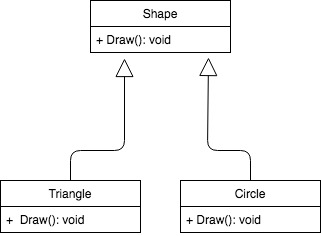
\includegraphics[scale = 0.80]{UML.png}
            \caption{Sample UML class diagram}
            \label{fig:my_label}
        \end{figure}
        
    \section{Class relations}
    From all your practices about class relations, there should be no more need of explaining the benefits of using inheritance in your project. Clever use of inheritance in your classes will save you from rewriting a lot of code from your projects as well as give you more flexibility on incorporating many kinds of objects, in a single data structure for example. Other kinds of class relations are \textbf{Association, Aggregation, Composition and Dependency}. How well you define these relationships and appropriate use of relationships depending on your use will also be an important criteria in judging your project.
    \section{Dividing work}
    Along with defining classes and relationships for your project, you will also be asked to show how this project will be divided among all team members. The UML can easily represent the work you divide and it is recommended that this information be conveyed in your UML through different colors, which improves readability. You may color each class by a color which represents a group member. It is important that at this stage, you have a clear idea about how much work each class is, as well as the weaknesses and strengths of your team so you can divide work accordingly. Similar classes should be awarded to the same person so that work can speed up.
    
    
    \section{Resources and tools}
    \begin{itemize}
     \item \color{blue} \href{https://www.visual-paradigm.com/guide/uml-unified-modeling-language/what-is-class-diagram/}{What is a class diagram?} \color{black} For a deeper understanding and tutorial for making your UML
     \item \color{black} UML creation tools:
     \begin{enumerate}
     \item \color{blue} \href{http://www.umlet.com/}{UMLet} \color{black}
     \item \color{blue} \href{https://www.gliffy.com/examples/uml-diagrams}{Gliffy} \color{black}
     \item \color{blue} \href{https://creately.com/Draw-UML-and-Class-Diagrams-Online}{https://creately.com/Draw-UML-and-Class-Diagrams-Online} \color{black}
     \item \color{blue} \href{www.lucidchart.com/}{www.lucidchart.com/} \color{black}
     \end{enumerate}
  
    \end{itemize}
     
     
%----------------------------------------------------------------------------------------
%	PART
%----------------------------------------------------------------------------------------  
    
    
\part{Visuals and Audio}

%------------------------------------------------
%	Chapter
%------------------------------------------------
\chapter{Designing Sprites} %Ahmed
    \section{Choosing sizes}
        \subsection{Game Screen}
        Scaling a game through multiple displays is always a tricky job. A certain size may be fitting the entire window in a 720p display but appears to be too small on a 1080p display. Simply increasing the size of your window is not a viable solution as that would cause it to overflow from the screen on smaller displays. It is therefore a good idea to fix your screen size to 1024 by 768 pixels which is a gaming standard and it is a much greater chance your window fits on the screen of your computer. If it is too small for your or your partner's display, you should reduce your screen resolution which would make the window appear larger on a higher resolution monitor. Figure 3.1 below will give you an idea about how different resolutions' sizes vary relative to each other.
        \begin{figure}[ht]
            \centering
            \includegraphics[scale = 0.58]{resolution.jpg}
            \caption{Resolution comparisons}
            \label{fig:my_label}
        \end{figure}
       
    \subsection{Sprites}
     To save memory and use it as efficiently as possible, it is a good idea to keep your graphics in a size that is a power of two. The size could vary for every object and game. It is important that the sprites have a transparent background without which no game can look good, if the backgrounds of the sprites are not transparent, you will be only available to render rectangles on the screen. For moving objects it you will have to make multiple sprites for them depending on how do they move, in general, the more frames for animation you create, the smoother your animation is. \newline
     While you may choose to not do so, all professional developers always design and produce their sprites in a much higher resolution than the resolution they need. For example, a sprite with dimensions 32*32 may be made originally in 512*512 size and then shrunk down. This results in a much higher quality image when shrunk to it's required size as the details it is designed in can be much greater. It also gives the advantage of being able to increase the size of the sprite later on as it is still being shrunk down from original instead of being expanded from a smaller size.
     
\section{Format}
        You should always store your images in the png file format as unlike jpeg, it allows backgrounds to be transparent, opaque or translucent.No background means that the inside the size that your image is, which is a rectangle, anywhere there is no image,for example, the region outside a circle that extra area is transparent and therefore it is whatever is below it.Without opaque backgrounds, your object can be of any shape, not just a rectangle which is a necessity for your project. There are a number of tools that you can use to remove a background and some of them are mentioned below, in the recourses and tools section. Figure 3.2 shows the effect of a transparent background.
        \begin{figure}[ht]
            \centering
            \includegraphics[scale = 0.58]{png_no_background.jpg}
            \caption{White vs transparent background}
            \label{fig:my_label}
        \end{figure}
        \newline
   You may realize this that it is never the case in any game or software that individual objects are rendered without a transparent background. If you are making your own graphics or downloading them from the internet, you should remove any background included in the image. One important point to remember here is that if an image has a transparent background (which is likely the case if you download sprites from the internet with a .png extension) opening and saving in MS Paint will make that background white, so never edit such images in paint, unless you can remove its background later.
        
    
    \section{Making your own vs Getting from the internet}
   If what you are trying to make has been done before and is popular, there is a good chance someone has uploaded it's recourses on the web. Unless you are skilled in it, making sprites from scratch is a very difficult job to do, one that may take dozens of hours depending on how detailed and many sprites you have. It is therefore a good idea to always search for sprites you want on the internet first. That said, even if you do find sprites you need, they may be not exactly what you want or more commonly, of very poor quality. You may need to edit some or even make new by yourself. Even if sprites may not be readily available, you may still easily find back drops for your project in very high quality on the internet so that is one thing you will not have to make on your own at the least. If you do find sprites that aren't as good as you wanted them to be, editing over them is still a better way to do it than completely making them on your own if time is your primary concern. The spritesheet for this project was made on Piskel which is an online tool, and there are many similar websites that help producing sprites and even show resultant animation of the sprite as well as have available, many sprites as templates. Before you start on your sprites, it is recommended that you atleast spend some time on the internet searching for your desired sprites. 
    \section{Sprite Sheet}
    Since your project will have many sprites, typically in the dozens, it is a much better idea to put all of your project sprites into a single image, which we will be calling the sprite sheet. There are many advantages of doing so:
    \begin{itemize}
    \item Sprite sheets load quicker since we do not need to load a new file every time we render object.
    \item A single image file will use less space since there will be only one header rather than dozens (there is alot of data stored in an image file other than just the pixels, this data is called a header).
    \item Individual sprites can be easily taken out so it does not complicate code either.
    \item The risk of putting in incorrect file names is drastically reduced.
    \item If there is an encoding error or you need to resize all your sprites, it becomes a much easier task to do.
    \end{itemize}
    Therefore, it is required by you to abide by the same procedures and maintain a single image file for all your sprites for this project. Your backgrounds and other similarly large images should be in a separate file however, since they are only being used once and then cleared from memory. All characters,numbers and buttons will also be included here.
    \begin{figure}[ht]
            \centering
            \includegraphics[scale = 1]{sprites.png}
            \caption{Sample Sprite sheet}
            \label{fig:my_label}
        \end{figure}
      
    \section{Buttons}
    In GUI, buttons are a very important form of user input. Our screens are flooded with buttons and you have probably never come across any application that doesn't contain buttons. For this reason, you shall also be required to use buttons in your project, especially on your home and your pause screen. Text will also be rendered on a button, not through a library but you will be rendering individual characters on each button. Your buttons should have three sprites associated with them,each representing three states. The first state is the default state which will be rendered when there is no mouse activity on the button, the second state is hover, which is active when the user's mouse is inside the button and the third sprite is rendered when the button is clicked. We will go through how to use the button later on in this guide. Buttons with all these three states can be easily found on the internet however, they will be more commonly available as a photoshop document, a simple search on Google "buttons.psd" should take you to numerous websites that have these available for free.
    \begin{figure}[ht]
            \centering
            \includegraphics[scale = 1]{button.png}
            \caption{Sample Button sprite}
            \label{fig:my_label}
        \end{figure}
        
        
    \section{Backgrounds}
    It is also required that you gather a plurality of background images for your project which fit your entire screen. You can easily find relevant images for your project on the internet. You will need to provide background graphics for your splash screen, your home screen, pause screen and exit screen, more on these screens later. You may choose to use the same images for all these screens although it is not recommended, more images aren't difficult to find nor add but they do look much nicer and add to the appeal of your project.
    
    
    \section{Resources and tools}
    \begin{itemize}
    
        \item \color{blue} \href{https://inkscape.org/en/release/0.92.3/}{Inkspace} \color{black} A picture editing tool
        \item \color{blue} \href{https://www.adobe.com/products/photoshop.html}{Photoshop} \color{black} A picture editing tool
        \item \color{blue} \href{https://www.youtube.com/watch?v=givuYd_cKm0&list=PL6gx4Cwl9DGD25IGk9Xf7oC3wiT9gC75x}{Photoshop CS6 by thenewboston
} \color{black} for a beginner's tutorial for photoshop
    	\item \color{blue} \href{https://www.freepik.com/}{https://www.freepik.com/} \color{black} contans many graphics in the psd format for easy editing and use.
        \item \color{blue} \href{https://www.piskelapp.com/}{Piskel} \color{black} A free and simple online sprite creator
        \item \color{blue} \href{https://brashmonkey.com/}{Spriter} \color{black} A more advanced sprite maker

    \end{itemize}
    
    
%------------------------------------------------
%	Chapter
%------------------------------------------------

\chapter{Using Sprites with SDL} %Aiman
    \section{LTexture class by LazyFoo}
    SDL offers a great texture rendering API which enables us to load texture and then render them to screen. There are SDL functions available that you can use to load the image and render them to screen at any position. \\  \\
    If you are learning SDL from LazyFoo tutorials, then you must have noticed that to make life easier, they have defined a separate class \textit{LTexture} for image loading and rendering purposes and doing all sort of stuff that you want to do with the image like color keying etc. Making a class would make it easier to do all these things rather than using SDL functions every time. \\    \\
    This class has a constructor/destructor pair, a loader function that loads the image from a file, a deallocator that frees the image, a renderer that takes in a position, and functions to get the texture's dimensions. \\   \\
    If you are starting to work on your project, then copy paste \textit{LTexture} class from LazyFoo tutorials, define separate header and \texttt{.cpp} for it and then continue loading images and rendering on screen. 
    \section{Loading sprites}
    By now you have probably some idea that we define and load texture in \texttt{loadMedia()} function in \texttt{main.cpp}. If you are working with \textit{LTexture} class, then you need to define LTexture's class object in main, and then call its image loader function \texttt{LoadFromFile(string filename)} in  \texttt{loadMedia()}  function. \\
    \pagebreak
    \begin{lstlisting}[language=C++, caption=Using LTexture to load images]
LTexture gSpriteSheet; //Ltexture's object

bool loadMedia()
{
	//Loading success flag
	bool success = true;
	if(!gSpriteSheet.LoadFromFile("Images/mySpriteSheet.png",gRenderer))
	{
		printf( "Failed to load sprite sheet texture!\n" );
		success = false;
	}
    return success;
}

\end{lstlisting}

    \section{Rendering Sprites}
    
This was just about loading an image. As discussed above, it is a good practice to put all of your images in a single sprite sheet to save memory. For this we will always load a single sprite sheet which will have images for all, for example, pacman, ghosts, candies and lollipops etc.\\ \\
In order to render any object, for example if you want to render a lollipop to screen, you will have to define an \texttt{SDL\_Rect spriteClip} as an attribute in \textit{Lollipop's} class that will define the \texttt{x, y} positions and  width and height of the part of the sprite sheet that you want to give to the object Lollipop. \\ \\
The \texttt{x, y, width, height} dimensions of the clip can be figured out using MS paint.
In the \textit{View} tab, check on \textit{gridlines} so that gridlines can appear on your image as shown in the image below. Now you can easily figure out the clip dimensions by hovering the cursor over the clip.
\begin{figure}[ht]
            \centering
            \includegraphics[scale = 0.82]{imageClip.JPG}
            \caption{Using MS paint to figure out clip dimensions}
            \label{fig:my_label}
\end{figure} \\ 
Now that you know the clip dimensions, you can specify the values for \texttt{SDL\_Rect spriteClip} in \textit{Lollipop's} constructor which will have the \texttt{Ltexture*} as a parameter so that it knows what image needs to be clipped. \\
\newpage
\begin{lstlisting}[language=C++, caption=Setting Sprite's dimensions; ]
Lollipop::Lollipop(LTexture* image,int x,int y):FoodItem(image,x,y)
{
    //ctor
    spriteClips.x = 385;
    spriteClips.y = 93;
    spriteClips.w = 32;
    spriteClips.h = 32;

    widthSheet = spriteClips.w;
    heightSheet = spriteClips.h;
    name = "LOLLIPOP";
}
\end{lstlisting} 

\noindent In order to render Lollipop, call LTexture's render in Lollipop's render funtion:

\begin{lstlisting}[language=C++, caption=Setting Sprite's dimensions; ]
void Lollipop::Render(long int& frame, SDL_Renderer* gRenderer)
{
    spriteSheetTexture->RenderTexture(position.x-widthSheet/2,
    position.y-heightSheet/2,gRenderer,&spriteClips, SDL_FLIP_NONE);
}
\end{lstlisting} 

\chapter{Audio}
    \section{Audio in a game}
    Audio is a very important aspect of a game. Audio together with graphics is what makes up the aesthetics of a game. \\ \\
    If you want to set up SDL Mixer, follow the instructions given in this link: \textcolor{blue}{\href{http://lazyfoo.net/tutorials/SDL/06_extension_libraries_and_loading_other_image_formats/index.php}{Setting up SDL Mixer}} \\
    If you are confused how to play sounds effects and music using SDL, then check out this link: \textcolor{blue}{\href{http://lazyfoo.net/tutorials/SDL/21_sound_effects_and_music/index.php}{Playing Sounds and music using SDL}} 
    
    \section{Resources and tools}
    Following links may be useful to find free sound effects and music for your game:
        \begin{itemize}
            \item \color{blue} \href{https://freesound.org/browse/tags/sound-effects/}{freesound} 
            %add more
        \end{itemize}  

%----------------------------------------------------------------------------------------
%	PART
%----------------------------------------------------------------------------------------

\part{Player(s) and other objects}
%------------------------------------------------
%	Chapter
%------------------------------------------------
\chapter{User input} %Ahmed
Without any form of input, your project will be basically nothing more than a video. User input needs to be handled very well and needs to be as easy for the user as possible. Your game can have any form of user input available. Most commonly it will be a combination of a keyboard and a mouse but you may choose to also include options for a joystick or even a touchscreen(necessary if you wish to develop for a mobile platform). For the sake of this guide, we will only focus on keyboard and mouse inputs. The tutorial on using mouse and keyboard is already present in the lazyfoo tutorials, which you were expected to already go through therefore this guide will skip ahead to some explanations and common traps for inputs and ways to avoid them.
    \section{Mouse}
    There are only two things you need to check when dealing with a mouse, it's state and it's position. All mouse events will be handled by SDL\_Event.
    \begin{lstlisting}[language=C++, caption=Getting mouse state]
SDL_Event e;
while( SDL_PollEvent( &e ) != 0 )
{
    if( e.type == SDL_MOUSEMOTION || e.type == SDL_MOUSEBUTTONDOWN
        || e.type == SDL_MOUSEBUTTONUP )
        {
            //Get mouse position
            int x, y;
            SDL_GetMouseState( &x, &y );
        }
}
\end{lstlisting}

The while loop will keep running until all registered poll events have been checked. It ensures that no event gets skipped during processing of the previous one. This code will give you the position of the mouse anytime it is moved or a button pressed or released. \\ \\
It is recommended that this be done in the main function. Lazyfoo passes a pointer to the SDL\_Event to the object, which doesn't make a difference if you have only one object but if you have many, objects, this strategy makes you redundantly check the mouse state. Therefore it is better you do this once in main and then either pass the mouse co-ordinates to each object to check if the activity is over that object or get the position of each object and check that in main. \\ \\
Either way, it would be incorrect to simply hard code positions to check for a mouse collision, below is an incorrect implementation :
\begin{lstlisting}[language=C++, caption=Checking incorrectly if a button is pressed ]
if(x>=70 && x<=470 && y>=137 && y<=217){
  if(event.type == SDL_MOUSEBUTTONDOWN){
   //your code here
   }
 }
\end{lstlisting}
This code checks if the mouse is clicked inside the dimensions of a button but the problem here is that this will have to be done for each object, moreover if the position or the dimensions of the button is changed, this piece of code will have to change as well, which becomes tedious and elements the purpose of using objects entirely, below is a sample code of how to do this correctly :
\begin{lstlisting}[language=C++, caption=Checking correctly if a button is pressed ]
if(button.isOverMouse(x,y)
{
  	if(event.type == SDL_MOUSEBUTTONDOWN)
    {
    	//your code here
    }
}
\end{lstlisting}
In this example button is an object for a Button and it has a function \texttt{isOverMouse(x,y)} that returns a \textbf{bool} value depending on whether the mouse co-ordinates are inside the limits of the button.\newline
The order of your \textit{if conditions} may be different depending on how you prefer or need.
    
    
    \section{Keyboard}
    When discussing keyboard inputs, there are two different methods that can be used. The first type is to use SDL\_Event and figure out which key was pressed. The other type is by using currentKeyStates which uses an array of all inputs to show which one is currently pressed. LazyFoo has tutorials for both of these methods.The first method uses a queue to store all key presses and therefore using this method ensures that all the keys pressed are registered and not missed. This method may be helpful in an application which requires something to be typed. However, this is not useful in making games and will most likely cause problems as a key pressed may register any number of unexpected additions to the queue and may cause delays in input and processing. currentKeyStates however show the keys pressed in real time so a key pressed is registered as long as it is pressed. This method also comes in much handy when checking for multiple key presses at the same time, which may be the likely case if you are building a game that has two players. Whichever method you choose, it is recommended that this checking for key presses be in your game's main loop. 
    
%------------------------------------------------
%	Chapter
%------------------------------------------------    
\chapter{Player} %Aiman
    \section{Assigning control to the player}
    One of the most important aspects of a game is the control assigned to a player. It may entirely depend on the type of the game whether the player should be given a complete and precise control, or a limited control. For example, for a soldier fighting game, a game developer may want to give the user or the player all the controls that a real soldier may have in real, or at least the main ones. But for a simple game like pac-man, where there's not much a player can do than just moving around for collecting/eating things, players only have limited controls such as movement in different directions. You can always add more control to your player according to the game.
    \section{Player Movements}
    A player should have a proper movement. It shouldn’t vibrate. It should have a steady movement. The shakiness causes the quality of the game aesthetics to fall and is unpleasant for the eyes. So the sprites must be chosen wisely especially for the animations.  \\ \\
    Furthermore, the player movements must be natural and logical. The player or the enemies shouldn’t pass through the walls or the floor/ceiling. They shouldn’t defy the laws of nature and physics, unless the game asks for it. Never call these bugs as features!
    \section{Camera}
    Camera is really important when it comes to show the point of view. It is what point of view of the game you want to focus more and it can become important when you want to shift the focus of the player from one thing to another. This obviously isn't the case with board games or maze games like pacman where the focus is only the board or the maze. 
    You should be very careful when changing the camera movements. For example, if camera screen is being moved to view a different perspective, it must be made sure that the camera movements are smooth and they are not unpleasant and shaky. 
    

%------------------------------------------------
%	Chapter
%------------------------------------------------
\chapter{Objects' interactions} %Aiman
    \section{Collision} %Aiman
    Your game starts to take real shape when you add collision within objects. In order to add collision, you can make your own collision function or you can even use SDL's intersection function \textcolor{blue}{\href{https://wiki.libsdl.org/SDL_IntersectRect}{SDL\_IntersectRect}} that returns  true if any of the object's rectangle intersect, otherwise false. If you haven't read Lazy Foo's collision detection lesson, then you must give it a read. \\ \\
   Checking for collision with objects may also increase complexity in a game. Like in a fighting game, you may need to check the collision of every bullet with every hittable object present in your game in every frame. If you have too many objects, then your game would become extremely slow. Rather you should always try to for effective techniques. An effective technique would be to divide the screen into a grid and checking the collision of the player with the object only within the nearest grid box so that bullets currently in first grid in a frame are checked with the elements of first grid only. \\ \\
   Even the sample game pacman uses an efficient technique. Rather than checking collsion of pacman with the food items of the entire grid in each frame, pacman only checks if there is a food item in it's current cell. It's current cell location is updated every time the character moves based on his direction.
    \section{Timed items} %Aiman
    Timed items are often called bonus items that are showed on the screen if a player plays well or if a certain time has elapsed. 
    Timed items may include an extra life pack, a sack of money, or any other item that may be important to the player. 
    
 

%----------------------------------------------------------------------------------------
%	PART 
%----------------------------------------------------------------------------------------

\part{Game}
%------------------------------------------------
%	Chapter
%------------------------------------------------
\chapter{Designing Levels} %Ahmed
\section{Fixed Levels}
Many games we play today have play today have fixed levels, meaning that the level layouts have been predeclared and saved in the code of the game. This is especially common in games that are story based. Implementing this popular approach will require you to design these levels in advance and test them out. Designing such levels would vary from each game, it may be the matter of designing mazes, obstacles, order of enemies or even tasks. \newline
These levels may be saved in the code of the game or as a saved state which will be discussed later on how to do that. If the instructions are saved in the code of the game, it will be hidden from the user and maybe more difficult to alter or add new levels depending on how you do it. \newline
If your game has fixed levels, the advantage may be a linear growth of difficulty as the levels progress but at the same time have this disadvantage that your game will be completed in a limited time, depending on how many levels can you program.
\newline
\newline
\textbf{Examples:} GTA, Pokemon Nintendo games, Mario, Angry birds
\section{Random levels}
Another approach to designing the layout of your game can be to generate levels randomly. This will most likely be more difficult than simply hard coding a level but will be more rewarding. The sample game provided to you generates levels randomly so it's code can be reviewed to better understand in detail possible ways of applying this approach. \newline
Random level generation doesn't literally mean generating the entire level randomly and being done with it. Rather, along with randomness there should be a set of very intelligent rules that give the game some playable sense. For example, if your game relies on a maze, it should be made sure there are no dead ends of areas that are completely surrounded by walls and therefore inaccessible. If you generate enemies randomly, and if there are many different levels of enemies, an algorithm should be implemented that give higher probability to the weaker ones as well as keeping check of a reasonable time span between which enemies spawn.
\newline
An important advantage of generating random levels is that your game is always different and you can generate all possible levels if you have mastered the random level generation. Unlike having fixed levels, randomly generating a level makes the game a bit more difficult as the user cannot anticipate the next level by simply playing the game again from 0.
\newline
Additionally, you may even generate levels randomly but fix their states by testing them all and deciding in their difficulty if that is what you would like to do.
\section{Endless level}
Perhaps most of the addictive mobile games available are based on an endless level scheme. These games do not have explicit stages and therefore do not give the user a sense of completion but rather push the player to continue playing \textbf{'endlessly'} to challenge himself and eventually beating only his highscore. These games do not require the additional effort to design multiple levels for the user to continue playing. These games are therefore based all around a scoring mechanism. As the level progresses, the difficulty of the game may implicitly increase to not let the user get bored once he has played enough of the game.
\newline
\newline
\textbf{Examples :} Flappy Bird, Subway Surfers, Sims city
\newline
\newline
\newline
Whichever method of game designing you choose, it is always a good idea to go through games of similar design to get a better understanding if implementing it, as you'll be learning through the products of professional game developers.
%------------------------------------------------
%	Chapter
%------------------------------------------------
\chapter{User interface} %Aiman
    \section{Screens}
    One of the most important aspects of a good video game is the user interface (UI) that it provides. A user interface is something by which the user can interact with the computer in order to play the game. Sometimes, some important information about the game needs to be shown to user. Sometimes, the user needs to give input to the computer to do different tasks such as restart, pause or exit the game. For this purpose we use different screens to handle different types of inputs and to show different information. \\
    \\
    A game may have many different screens, for example a splash screen, a menu screen, an excerpt screen, a game screen (the main playing screen), a pause screen, and and an exit screen and if necessary, a game over screen to show that the player has lost the game or a winning screen if the levels are not endless. A video game can have more screens depending upon the implementation and the requirement of the game. Since all these objects are all screens just with different purposes and layouts, the best class design would be to create an abstract \texttt{Screen} class (because a screen's object will not be created, only its child classes will be declared as as objects in \texttt{main.cpp}, and inherit all other types of screens from this base class. \\ \\
    The game provided you as a sample contains the following screens.
\subsection{Splash Screen}
        A splash screen is a graphical control element consisting of a window containing an image, a logo, and the current version of the software. A splash screen usually appears while a game or program is launching. \\  \\
A splash screen is a simple class where only the rendering of the image takes places.
It is shown for a very short span of time after which transition to menu screen takes place.
\subsection{Menu Screen}
Menu screen is an interface that allows the player to choose between options necessary for playing a game. A simple menu screen may consist of a \textit{New Game} button to start a new game, a \textit{Continue Game} button to load a saved game or an \textit{Exit} button to exit the game. It may however also include options for players such as choosing between single player or multiplayer, or choosing the difficulty level etc. 
\begin{figure}[ht]
            \centering
            \includegraphics[scale = 0.4]{main_menu.JPG}
            \caption{Sample Game's Menu Screen}
            \label{fig:my_label}
\end{figure} 
\subsection{Excerpt Screen}
An excerpt screen is  used to display any important information that the player should know before playing a game. You can also show the instructions (what the player has to do in that game) or the story of the game in an excerpt screen, or you can make a separate screen for instructions which can be accessed through \textit{Instructions} button in menu screen.
 \begin{figure}[ht]
            \centering
            \includegraphics[scale = 0.4]{excerpt.JPG}
            \caption{Sample Game's Excerpt Screen}
            \label{fig:my_label}
\end{figure} 
\subsection{Game Screen}
This is the main playing screen. This often contains necessary options that are required while a game is being played such as a \textit{Pause} button. A pause button gives access to pause screen. Some necessary information is also shown on the game screen such as the current score, level number being played or any other information related to the game like lives remaining, status of health bar etc.
\begin{figure}[ht]
            \centering
            \includegraphics[scale = 0.4]{game_screen.JPG}
            \caption{Sample Game's Game Screen}
            \label{fig:my_label}
\end{figure} 
\subsection{Pause Screen}
Pause screen is an important screen in a game. A \textit{Pause} button in game screen is used to access this screen. Some necessary functions or buttons that a pause screen should contain are: 
\begin{itemize}
\item \textit{Resume} button to continue playing the game.
\item \textit{Restart} button to start the game again.
\item \textit{Quit} button to give access to quit screen.
\end{itemize}
Your pause screen may also contain some special functionalities such as options for mute/unmute, or \textit{Control} button to show a screen displaying or changing the controls of the game etc.
\begin{figure}[ht]
            \centering
            \includegraphics[scale = 0.4]{pause_screen.JPG}
            \caption{Sample Game's Pause Screen}
            \label{fig:my_label}
\end{figure} 
\subsection{Exit Screen}
An exit screen or quit screen is usually accessed via \textit{Quit} button in pause screen. It is used to quit the game but with an added functionality of saving a game.  Some necessary functions or buttons that an exit screen should contain are: 
\begin{itemize}
\item \textit{Yes} button to save and then quit.
\item \textit{No} button to quit without saving.
\item \textit{Cancel} button to resume playing the game.
\end{itemize}
\begin{figure}[ht]
            \centering
            \includegraphics[scale = 0.4]{exit_screen.JPG}
            \caption{Sample Game's Exit Screen}
            \label{fig:my_label}
\end{figure} 
\subsection{Game Over Screen}
This screen is rendered when a player loses the game. It usually shows the highest score of the player, the score of the last game played etc. You can also make a game winning screen similarly if the game does not have endless levels.
\begin{figure}[ht]
            \centering
            \includegraphics[scale = 0.4]{game_over.JPG}
            \caption{Sample Game's Exit Screen}
            \label{fig:my_label}
\end{figure} 
\section{Scoring}
%------------------------------------------------
%	Chapter
%------------------------------------------------
In games, score refers to an abstract quantity associated with a player or team. Score is usually measured in the abstract unit of points, and events in the game can raise or lower the score of different parties. Most games with score use it as a quantitative indicator of success in the game, and in competitive games, a goal is often made of attaining a better score than one's opponents in order to win. \\
\\
Usually the score of a game have relevance to game play. In fighting games, for example, scoring a very high number of points could result in unlock-able players or modes or they can unlock the next level like in the sample game. In some games, reaching certain scores gives an extra life, or a continue. All this depends on the type of the game. There is often a time bonus which can add extra points.   \\
\\
In other games, points are typically gained from defeating monsters and enemies. When defeating a boss, a proportionally large number of points is usually rewarded. Extra points can be gained from gathering items, such as power-ups or other pick-ups. \\ 
\\
Usually, when a player gets a certain number of points, they may get an extra life or go on to a higher level. Points can be often used as currency which can redeemed for rewards and player upgrades.
\chapter{Save/Load} %Aiman
    \section{Game Save}
    \subsection{Saving in a \texttt{.txt/.csv} file}
    One of the easiest ways of saving a game's progress is to save the state of all the variables of the game (that are important to load afterwards) in a \texttt{.txt} or \texttt{.csv} file. All you need to know is how to write to a \texttt{.txt/.csv} file in c++, and save all the necessary information like the player's position, its health status, the score of the game, enemy positions and their health etc. in the file. Use an object's getter functions to save states for them. Below is a function for saving game. \\
\begin{lstlisting}[language=C++, caption=Saving a game]
void Game::SaveGame()
{
    std::ofstream file;
    file.open("GameData.csv");
    file << /* save any variable's state */ << "\n";
    file.close();
}
\end{lstlisting}
Sometimes, the information to store is often lengthy. Consider the example of the sample game provided to you. Since the levels are randomly generated, saving a game will also require you to save the level. Each level is a 2D array of Cells of dimension \(22 \times 32\). Each cell contains some information about it, whether it has a wall or any fooditem (candy or lollipop), is it restricted to not have any walls? Storing all these states for all \(22 \times 32\) cells can be very lengthy. Instead, one should go for easier ways that will require lesser effort to save. Since we need to store some information about each cell, give each information a symbol. For example: \\
\begin{itemize}
\item A cell filled with wall will have a symbol: “|\_|”
\item A cell which is restricted to have a wall will have: “x”
\item A cell containing a candy will have: “*”
\item A cell containing a candy will have: “**”.
\end{itemize} 
This will make a lot easier for the data to be stored. So the data about the entire maze can saved in a .csv file as:
\begin{figure}[ht]
            \centering
            \includegraphics[scale = 0.7]{maze_save.JPG}
            \caption{Storing information about maze/level}
            \label{fig:my_label}
\end{figure} 
The problems can arise when someone tries to modify this file which can cause problems. Players can also edit the file to hack the game and customize anything that may help them in winning the game. One way to avoid hacking is to avoid labeling the variable's state that you will save. So that no one knows what the values in the file actually represent. 

    \section{Game Load}
    One saving game has been done, loading a game is not difficult at all. It is only a matter of setting your variable's according to the file data after reading the file previously saved. \\
    \begin{lstlisting}[language=C++, caption=Loading a game]
void Game::LoadGame()
{
    ifstream file ("GameData.csv");
    string line;
    if (file.is_open())
    {
        getline(file, line);
        //load the level number of the game played last time
        level_no = atoi(line.c_str());
        //now close the file
        file.close();
    }
}
\end{lstlisting}

\end{document}
